 \chapter{Introduction}


Code-breaking games (sometimes also called \emph{deductive games} or \emph{searching games})
  are games for two players in which the first,
  usually referred to as \emph{the codemaker},
    chooses a secret code from a given set, and the second,
  usually referred to as \emph{the codebreaker},
    strives to reveal the code by a series
    of experiments that give him partial information about the code.

\begin{wrapfigure}{r}{0.32\textwidth}
  \vspace{-5mm}
  \begin{center}
  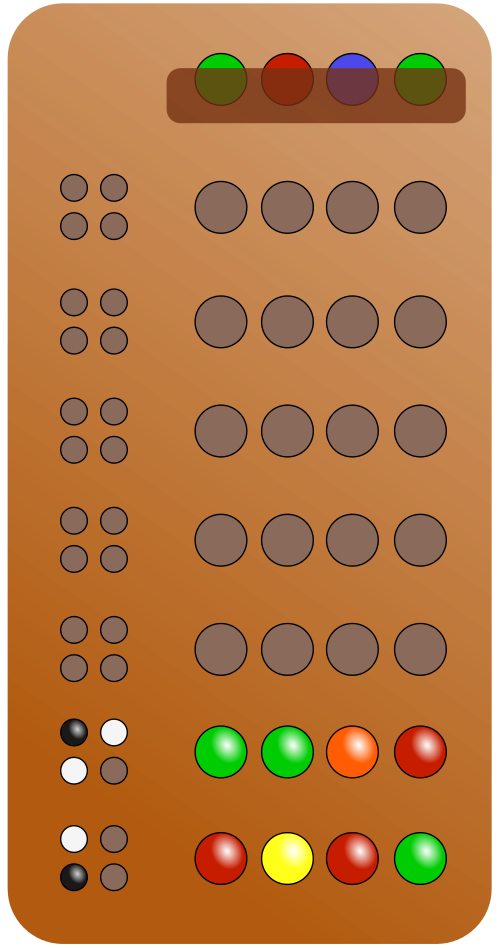
\includegraphics[width=0.25\textwidth]{pictures/mastermind.png}
  \vspace{-5mm}
  \end{center}
  \caption{Mastermind game (illustrative image)\protect\footnotemark.}
  \vspace{-5mm}
\end{wrapfigure}
\footnotetext{Image adopted from \url{http://commons.wikimedia.org/wiki/File:Mastermind\_beispiel.svg}, by Thomas Steiner under GFDL.}

The famous board game of \emph{Mastermind} is a prominent example.
The codemaker creates a puzzle for the codebreaker by choosing a
  combination of 4 coloured pegs (with colour repetitions allowed).
The codebreaker makes guesses, which are evaluated by the codemaker with
  black and white markers.
A black marker corresponds to a position at which the code and the guess matches.
A white marker means that some colour is present both in the code
  and in the guess but at different positions.

Another example is the \emph{counterfeit coin problem},
  the problem of identifying an odd-weight coin among
  authentic ones using just a balance scale.
The codemaker is not a real player here; the balance scale takes his function
  and evaluates the weighings performed by the codebreaker.
Numerous other examples can be found among various board games and logic puzzles,
 some of them being presented in the next chapter.

Code-breaking games bring many interesting problems to study.
Most importantly,
 \emph{how should the codebreaker play in order to minimize the number of experiments
   needed to undoubtedly determine the code?}
 \emph{Is there a strategy that would guarantee
   revealing the code in at most $k$ steps?}
 \emph{What strategy is optimal with respect
   to the average-case number of experiments,
   given that the code is selected
   from the given set with uniform distribution?}

Synthesis of an optimal strategy is a task computationally very intensive.
In some games, the optimal strategy might have a simple
  structure and can be described easily, such as in
  the counterfeit coin problem (see section \autoref{s:coins} for details).
In general, however, the strategy may have arbitrary structure and the only way
  to discover an optimal strategy is by considering all possible experiments
  in a given state and analysing the subproblems.

Therefore, one may prefer a suboptimal strategy or heuristics
  for experiment selection,
  which is easier to compute.
This brings another kind of problems.
Given a strategy,
  how can we compute the worst-case and the average-case number
  of experiments the strategy needs to reveal the code?

Mastermind and the counterfeit coin problem have been subjected to
heavy research and most of these questions are at least partially answered.
The exact results and summarization of the research in this area is presented
  in \autoref{ch:games}.
Nevertheless, few have been written about code-breaking games in general.
Some authors suggested general methods (and applied them on one of the games,
  e.g. \cite{cbg-stgopt, cbg-gen}),
  some vaguely stated that their approach can be applied
  to other games of the same kind but,
  to the best of our knowledge, no one has tried to
  create a general framework and provide
   results for code-breaking games in general.

Here comes this work to fill the gap.
We develop a general formalism that uses propositional logic to
  represent the secret code and the partial knowledge.
In short, the secret code is encoded as a valuation of
  a set of propositional variables
  and the codebreaker's goal is to discover the valuation
  using a series of experiments.
Each experiment can result in several outcomes,
  which are given in the form of a prepositional formula.

We study strategies for the games in general, with a focus on
  a special class of \emph{one-step look-ahead} strategies,
  strategy analysis and synthesis of an optimal strategy.
For these problems to be computationally feasible, one need to exploit
  symmetries of the game and neglect symmetric experiments during the analysis
  or strategy synthesis.
Algorithms for symmetry breaking in Mastermind
  based on graph isomorphism has been suggested in \cite{cbg-nauty}.
We generalize this approach and present
  an algorithm for elimination of symmetric experiments
  in general code-breaking games.

Main part of this thesis is a design of a computer language for
  code-breaking game specification
  and development of a computer program that
  loads a game from a file in the defined format
  and performs various tasks with the game.
We named the tool COBRA, the code-breaking game analyser.
Currently supported tasks are
\begin{itemize}
\item verify that a game specification is correct
  and sensible (overview mode),
\item simulate the game either interactively, with input from the user, or
  with decisions by specified strategies (simulation mode),
\item analyse a given strategy for experiment selection --
  compute the worst-case and average-case number of experiments needed (analysis mode),
\item synthesize the worst-case or average-case optimal strategy (optimal mode).
\end{itemize}
Using the tool, we can easily reproduce some of the known results
  for Mastermind and evaluate the same ideas in other code-breaking games.

The thesis is structured as follows.
Chapter 2 introduces several examples of code-breaking games,
  discusses known results, variants of the games and related research.
The general formalism, definitions and symmetry breaking approach
  are described in Chapter 3.
Chapter 4 is dedicated to our tool, COBRA, with description of its usage and
  abilities.
Experimental results with comparison of analysed strategies
  are presented in Chapter 5.
Finally, Chapter 6 concludes the work with many suggestions on future work
  and possible extensions of the tool.






